\documentclass{article}

% Language setting
% Replace `english' with e.g. `spanish' to change the document language
\usepackage[english]{babel}

% Set page size and margins
% Replace `letterpaper' with `a4paper' for UK/EU standard size
\usepackage[letterpaper,top=2cm,bottom=2cm,left=3cm,right=3cm,marginparwidth=1.75cm]{geometry}

% Useful packages
\usepackage{amsmath}
\usepackage{graphicx}
\usepackage{appendix}
\usepackage[colorlinks=true, allcolors=blue]{hyperref}
\usepackage{caption}
\captionsetup{justification=centering}

\title{Airframe Optimization}
\author{Ryan Howell}

\begin{document}
\maketitle

%\begin{abstract}

%\end{abstract}

\section{Introduction}

Through reading the textbook and SNOW.jl documentation as a part of this assignment, I learned about optimization processes and how to set up optimization problems using SNOW.jl. By experimenting with SNOW.jl inputs, I observed the aerodynamic effects of wing shape, particularly when optimizing for drag. In this report, I will discuss some key takeaways from the reading and explore the optimization process and resulting wings when varying specific parameters. These results will be explained using theory and compared to previous projects.

\section{Background Readings}
The suggested readings included a basic overview of the design process, with some focus on the actual optimization. It also went through the required setup to use the SNOW.jl optimization wrapper and its capabilities.

\subsection{Design Process}
The design process requires that an initial design be set, then evaluated, modified, and iterated until a good or optimal design is achieved. With an optimization algorithm, this iterative design can be repeated more quickly and find a better solution in most cases than repeated hand calculations. It requires the optimization problem to be formulated, with constraints, an optimized parameter, and input variables. 

\subsection{SNOW.jl}
To optimize in the SNOW.jl wrapper, the number of constraints must be set with upper and lower bounds, typically negative infinity to zero. The constraints are then defined in the function being optimized. The input parameters for the function also need to be defined with a range of potential values and an initial starting value. Once these are done, the minimize function can be called to optimize the design parameters for the given objective.

\section{Optimized Airframe Design}
Building off the airframe analysis of the previous report, I used the Vortex Lattice method to set up an optimization problem to find the best wing shape.

\subsection{Chord Distribution}
The primary problem and objective of this project was to optimize the chord distribution of a wing. This is accomplished by using the vortex lattice method to approximate the lift and drag of a wing in a function optimized with the SNOW.jl wrapper. Minimizing drag and maintaining a required lift of 1.7 pounds, while other constraints hold the wings to a reasonable shape. Such constraints include making sure the chord length decreases in size across the span of the wing and limiting how much it varies between sections to a reasonable amount based on the number of sections. This maintains a realistic wing that meets the operating conditions for the plane while reducing the drag on the wing, or the required thrust.

\subsubsection{Changing the Number of Sections}
Changing the number of sections allowed for increased refinement, as seen by comparing Figures \ref{fig:Low Res} and \ref{fig:High Res}. This creates a more accurate representation of the optimized wing. However, too many sections slow down the optimization significantly without much-added benefit or resolution. As you can see in the refined wing profile, the optimized planform area is very elliptic. The main deviation comes at the tip where it abruptly ends flat. This is to avoid the sharp increase in lift coefficient predicted by vortex lattice for wings with sharp tips, as shown in the last report.

\begin{figure}[h]
\centering
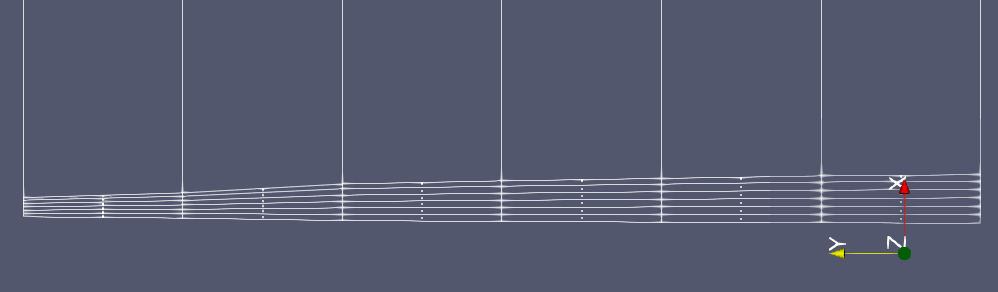
\includegraphics[width=\textwidth]{LOW RES FOCUSED.png}
\caption{Optimized wing of 6 sections}
\label{fig:Low Res}
\end{figure}

\begin{figure}[h]
\centering
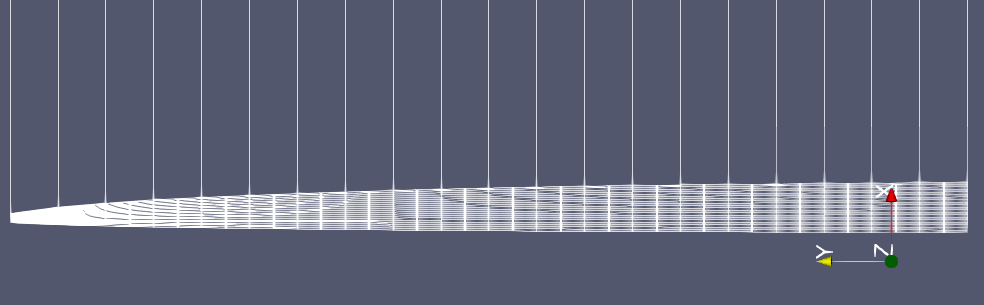
\includegraphics[width=\textwidth]{HIGH RES FOCUSED.png}
\caption{Optimized wing of 20 sections}
\label{fig:High Res}
\end{figure}

\subsection{The Effect of Constraints}
Upon finding this optimal wing chord distribution, the restrictions on the change in chord from one section to the next were removed, leaving only the lift restriction. Inputting the previously found chord distribution as the initial starting point, it converged to the same solution, shown in Figure \ref{fig:High Res}. Then I varied the lift constraint by changing the weight of the aircraft. This had a drastic effect on the wing lift distribution. As you can see in Figure \ref{fig:Slightly Higher}, when adding 4 pounds to the lift constraint, the wing chord starts to lengthen. When you increase the lift constraint by a factor of five, the chords lengthen even more, see Figure \ref{fig:5 Higher}. This is to create more lift, although it maintains its elliptical shape. With these larger wings, they look remarkably similar to the wings of a Supermarine Spitfire. The main difference being in the wingtips due to Vortex Lattice limitations as previously discussed. Increasing the weight of the plane also increased the time needed to optimize the problem.

\begin{figure}[h]
    \centering
\begin{minipage}[b]{0.45\textwidth}
\centering
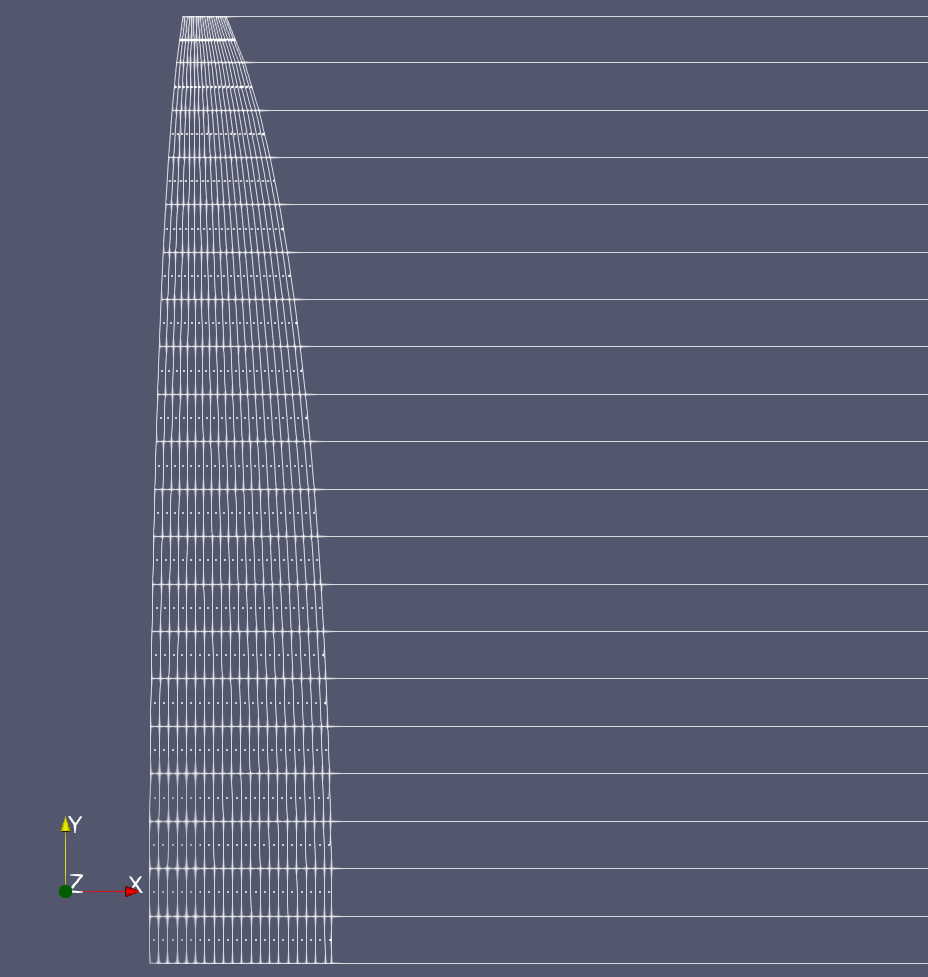
\includegraphics[width=\textwidth]{4 pounds more.png}
\caption{Optimized wing with 4 additional pounds}
\label{fig:Slightly Higher}
\end{minipage}
\begin{minipage}[b]{0.45\textwidth}
\centering
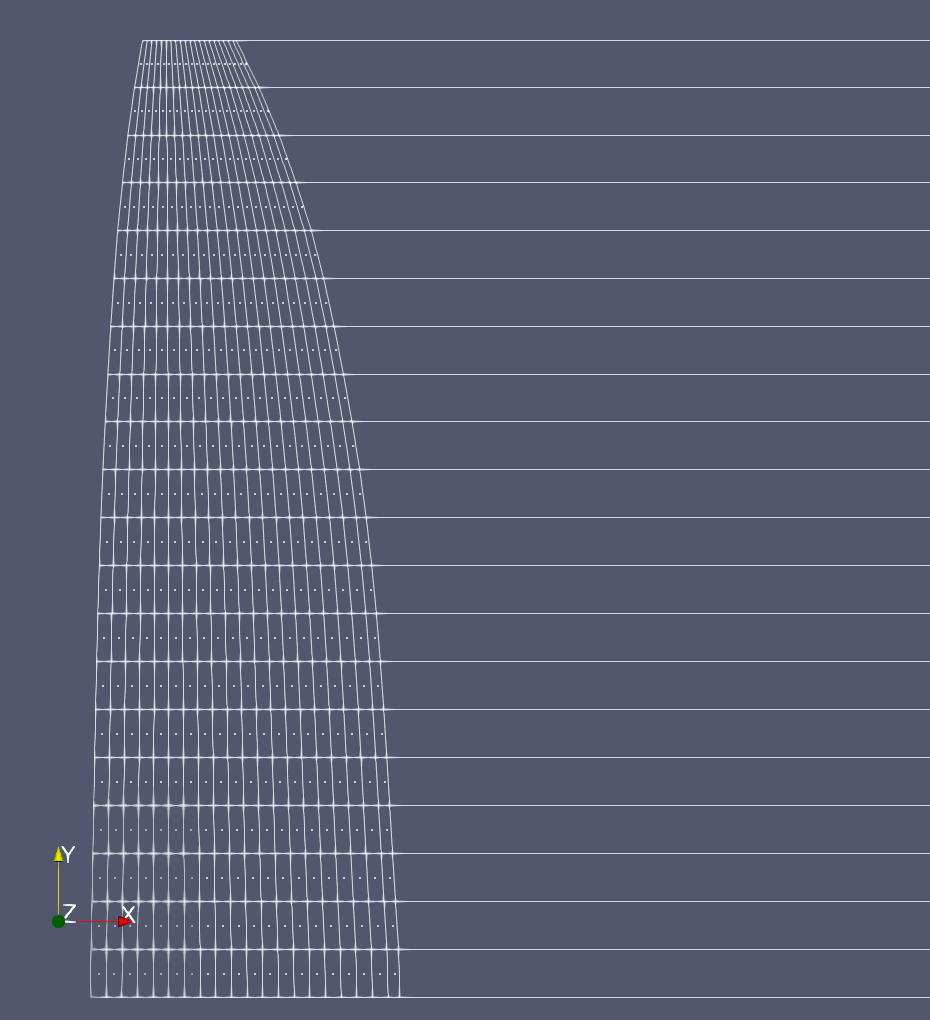
\includegraphics[width=\textwidth]{5 Times load.png}
\caption{Optimized wing with 5 times the load}
\label{fig:5 Higher}
\end{minipage}
\end{figure}

\subsection{The Effect of the Tolerance}

Increasing the lift constraint eventually leads to unsolvable scenarios, resulting in square wings or, through repeated iterations, partially square and elliptic wings but never converging to a solution. This can be reduced by increasing the tolerance as it allows for the optimizer to run more quickly and reduce how finely it searches for an answer. Then, using the optimized chord distribution from previous iterations as an initial point, you can decrease the tolerance until an adequate tolerance is achieved.

\section{Different Optimization Problems}

To gain increased and deepened familiarity with optimization problems and using the SNOW.jl wrapper, I completed the two additional optimization problems in the appendix of the handout. The first added a second variable that I optimized for, the angle of attack or pitch. The latter optimized the twist of the wing holding the chord constant.

\subsection{Varying Angles of Attack Along with Chord Distribution}
In this optimization problem, I had to pass in all the variables as one vector. This meant I had to separate the chords from the alpha value in the function. Once done, I could optimize the chord distribution and alpha angle separately. Interestingly, in the results, as shown in Figures \ref{fig:Optimized Alpha Small Load} and \ref{fig:Optimized Alpha Large Load}, the root chord varied by significantly less. The angle of attack was optimized to produce more lift while minimizing drag further. This led to a larger root chord at the normal lift requirement, 1.7 pounds, and a smaller root chord at 5 times that lift requirement. Compare Figures \ref{fig:Optimized Alpha Small Load} and \ref{fig:Optimized Alpha Large Load} with \ref{fig:High Res} and \ref{fig:5 Higher} respectively to see these differences. As noted in the captions of the images, the angle of attack increases with weight. This intuitively makes sense as a higher angle of attack will produce more lift while adding some drag. Using the Vortex lattice method will add some inaccuracies at high alpha angles of attack as it doesn't account for stall. This was minimized by setting up the optimizer problem with a max alpha of around 15 degrees, which is near the stall angle of most airfoils.

\begin{figure}[h]
    \centering
\begin{minipage}[b]{0.45\textwidth}
\centering
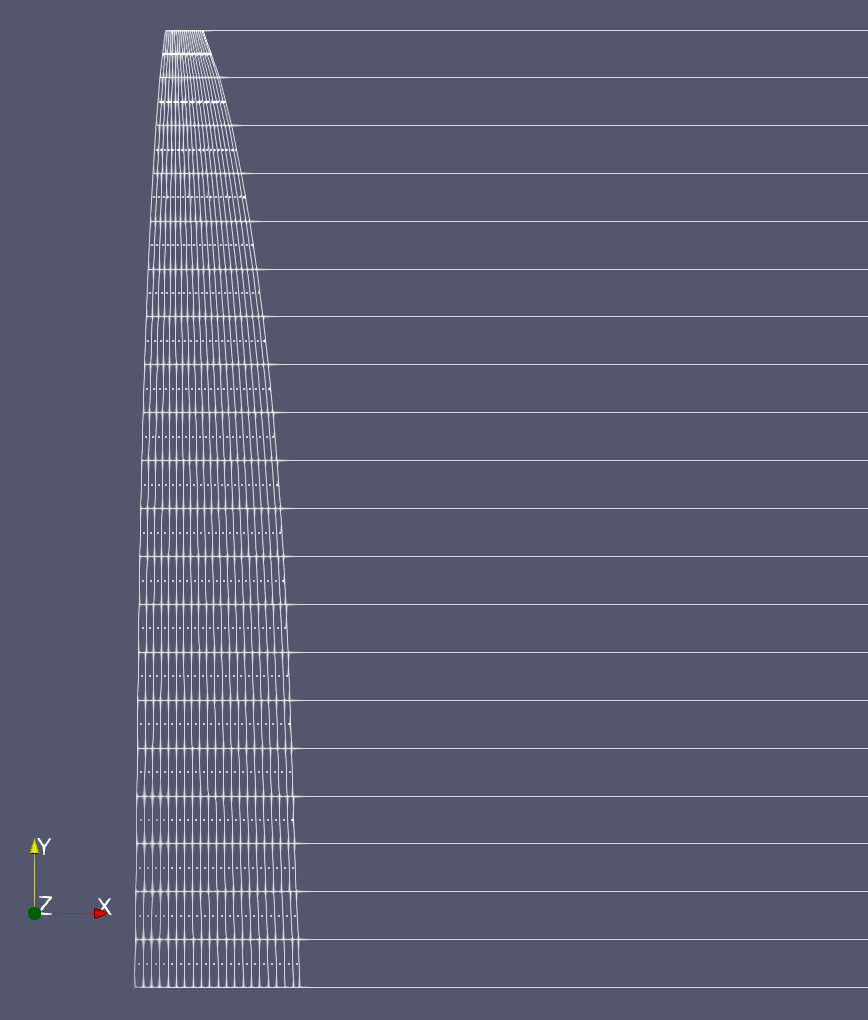
\includegraphics[width=\textwidth]{1 scale optimized alpha.png}
\caption{Optimized wing for base lift constraint and an optimized alpha of about 1.7 degrees}
\label{fig:Optimized Alpha Small Load}
\end{minipage}
\begin{minipage}[b]{0.45\textwidth}
\centering
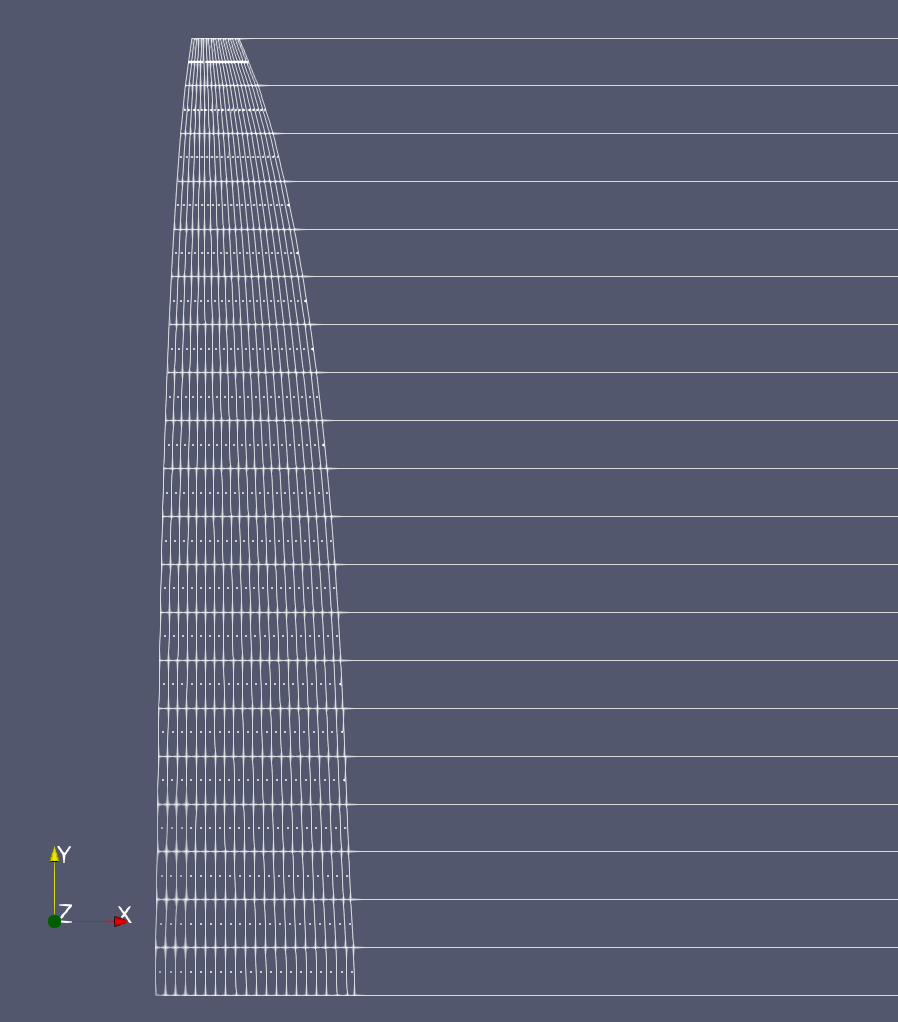
\includegraphics[width=\textwidth]{5 scale optimized alpha.png}
\caption{Optimized wing with 5 times the load and an optimized alpha of about 7.2 degrees}
\label{fig:Optimized Alpha Large Load}
\end{minipage}
\end{figure}

\subsection{Varying Twist Angle}
For this problem, I changed the chord distribution to be constant across the whole span of the plane. The optimizer then optimized the theta vector to reduce drag and maintain the requisite lift. For a larger rectangular wing, this produced relatively little twist, as some twist does help with drag. However, at higher weights, the optimal wing had more twist as this increases the amount of experienced lift, compare Figures \ref{fig:Optimized Twist Small Load} and \ref{fig:Optimized Twist Large Load}. This could be implemented with varying chord lengths to create an overall more optimal wing.

\begin{figure}[h]
    \centering
\begin{minipage}[b]{0.45\textwidth}
\centering
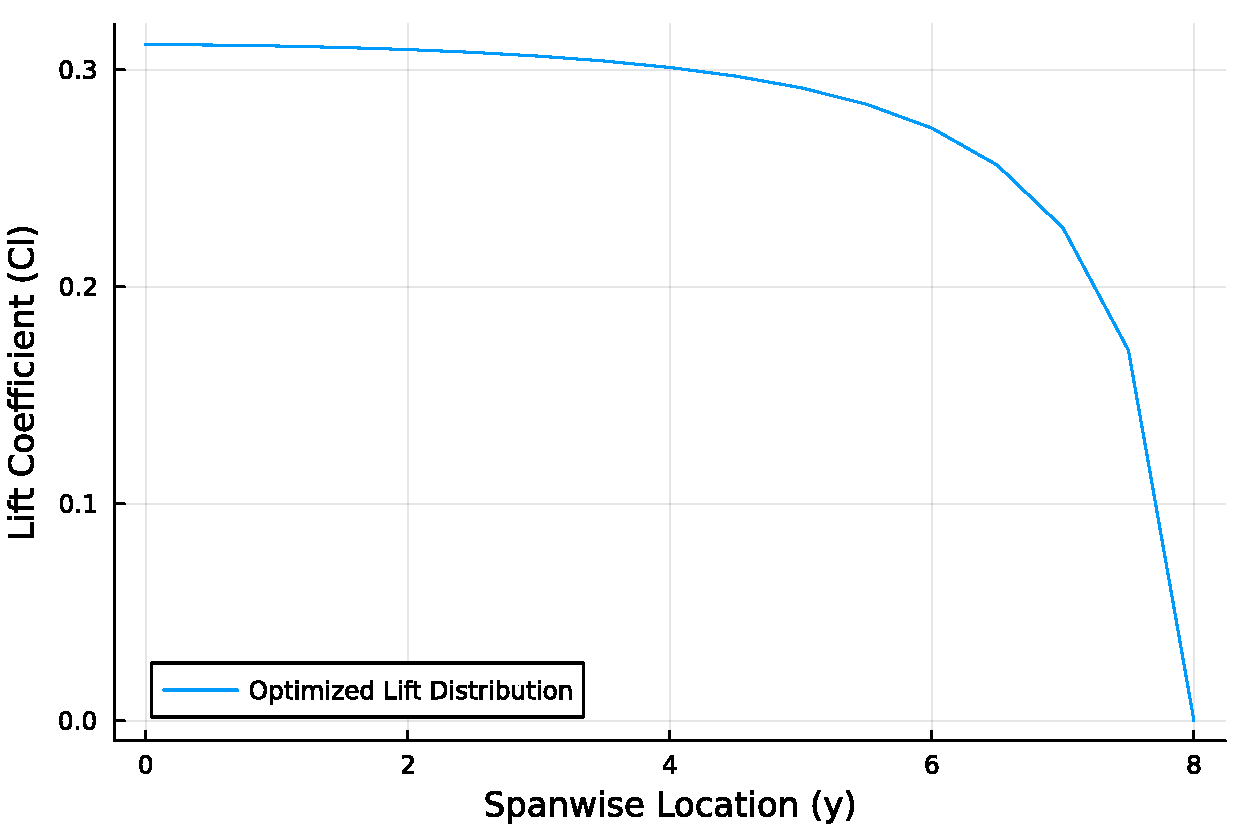
\includegraphics[width=\textwidth]{Lift_Distribution_along_the_Span_Twist_Optimization.pdf}
\caption{Lift distribution of a twisted rectangular wing}
\label{fig:Optimized Twist Small Load}
\end{minipage}
\begin{minipage}[b]{0.45\textwidth}
\centering
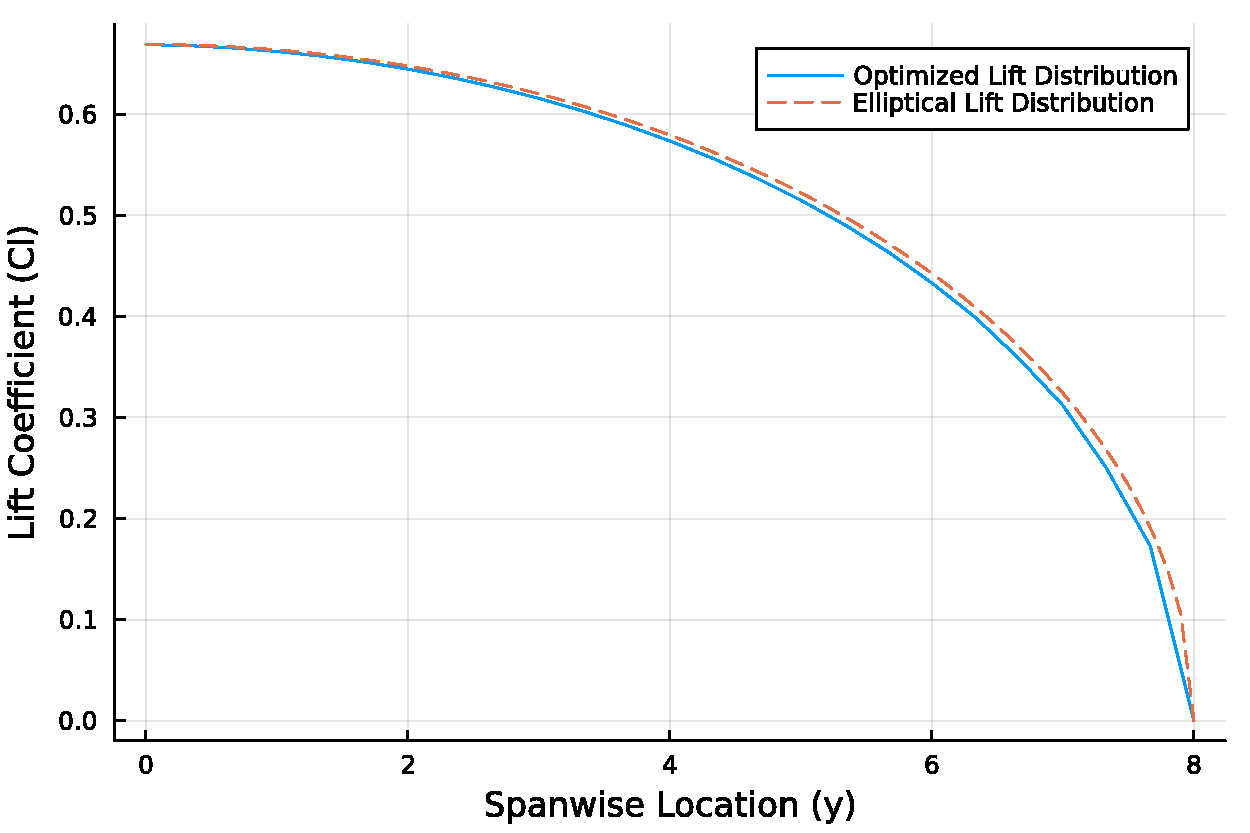
\includegraphics[width=\textwidth]{Lift_Distribution_along_the_Span_Twist_Optimization_increased_lift.pdf}
\caption{Lift distribution of a twisted rectangular wing with increased weight}
\label{fig:Optimized Twist Large Load}
\end{minipage}
\end{figure}

%\bibliographystyle{alpha}
%\bibliography{sample}

%\clearpage
%\appendix
%\chapter{Appendix A}

\end{document}